
\documentclass[aspectratio=169]{beamer}
\setbeamertemplate{navigation symbols}{}

\usepackage{subfigure,epsfig,amsfonts}
\usepackage{beamerthemeshadow}
\usepackage{amsmath}
\usepackage{bm}
\usepackage{siunitx}


\setbeamertemplate{footline}{}
\setbeamertemplate{navigation symbols}{}

\begin{document}
\title{Stochastic computation in recurrent networks of spiking neurons}  
\author{Clayton Seitz}
\date{\today} 

\maketitle


\begin{frame}{Outline}
\tableofcontents
\end{frame}

\section{Deep learning in a nutshell}

\begin{frame}{A brief survey of deep learning architectures}

\begin{itemize}
\item Perceptrons e.g. MLPs for classification of vectorized data
\item Convolutional neural networks (CNNs) for image classification, segmentation
\item Recurrent neural networks (RNNs) for temporal data
\item Generative adversarial networks (GANs) and autoencoders e.g. VAEs for generative modeling
\item ...
\end{itemize}

\vfill
{\color{red} which are all trained offline on known samples from some (perhaps very complicated) population distribution}

\end{frame}

\begin{frame}{What \emph{is} a deep network?}

Frank Rosenblatt, using the McCulloch-Pitts neuron and the findings of Donald Hebb, went on to develop the first perceptron
\vfill

Say there exists a set $\mathcal X$ of possible inputs and some set $\mathcal Y$ of possible outputs,
and a parameter vector $\Phi \in \mathbb{R}^d$.

\vfill
For $x \in \mathcal X$ and $y \in \mathcal Y$ a deep network $\Phi$ computes a conditional probability {\color{red} $P_\Phi(y|x)$}.
\end{frame}

\begin{frame}{A general prescription for training a deep network}

We assume a ``population'' probability distribution $\mathrm{Pop}$ on pairs $(x,y)$.

\vfill
\begin{eqnarray*}
{\color{red} \Phi^*} & {\color{red}  =} & {\color{red} \underset{\Phi}{\mathrm{argmin}} \;{\mathcal L}(x,y,\Phi)}
\end{eqnarray*}

\vfill
where $(x,y)\sim \mathrm{Pop}$. Learning (minimizing loss) occurs by some form of gradient descent e.g. stochastic gradient descent (SGD).

\begin{equation*}
\Delta \Phi = -\eta\frac{\partial \mathcal{L}}{\partial \Phi}
\end{equation*}

\end{frame}


\begin{frame}{Training large neural networks is computationally expensive}

\begin{itemize}
\item The entire brain is estimated consume 10W of power
\item Spiking networks (SNNs) perform computations in memory giving low-latency
\item SNNs can in principle self-organize without backprop (unsupervised learning)
\end{itemize}

\begin{figure}
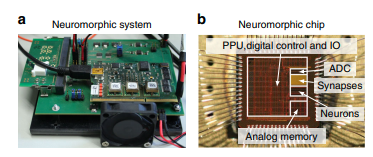
\includegraphics[width=110mm]{hardware-figure}
\end{figure}

\end{frame}

\section{Biologically inspired neural networks}
\begin{frame}{The third generation of neural networks: spiking nets}

\begin{columns}
\column{0.5\linewidth}
\begin{figure}
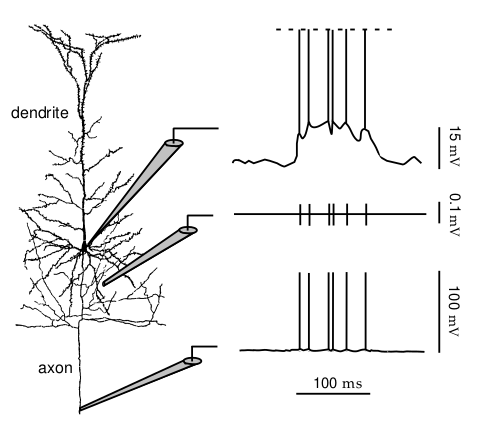
\includegraphics[height=55mm, width=75mm]{figure-18}
\end{figure}
\column{0.5\linewidth}
\begin{itemize}
\item $\sim$ 16 billion neurons in cortex
\item A neuron receives on the order of $10^{3}$ to $10^{4}$ synaptic inputs
\item Neurons communicate via action potentials in an all-or-nothing fashion
\end{itemize}

\end{columns} 

\end{frame}

\begin{frame}{The third generation of neural networks: spiking nets}

\begin{itemize}
\item Post-synaptic potentials (PSPs) allow pre-synaptic action potentials to change post-synaptic membrane potential
\item PSPs can be positive or negative (excitatory or inhibitory)
\end{itemize}


\end{frame}

\begin{frame}{Integrate and fire (IF) neuron models}

\begin{figure}
\centering
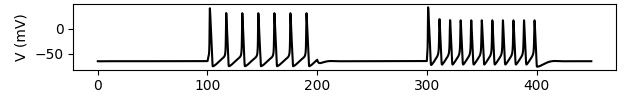
\includegraphics[width=140mm]{figure-19-1}
\end{figure}

\begin{figure}
\centering
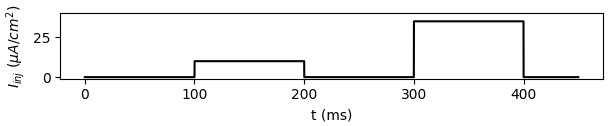
\includegraphics[width=140mm]{figure-19-2}
\end{figure}

\begin{equation*}
\tau\dot{V}(t) = g_{\ell}(E - V) + g_{\ell}\cdot \psi(V) + I(t)
\end{equation*}


\end{frame}

\begin{frame}{Monte-Carlo simulation of uncoupled IF neurons}

When $\psi(V) = g_{\ell}\Delta_{T}\exp\left(\frac{V-V_{L}}{\Delta_{T}}\right)$ we have the exponential integrate and fire model

\begin{figure}
\centering
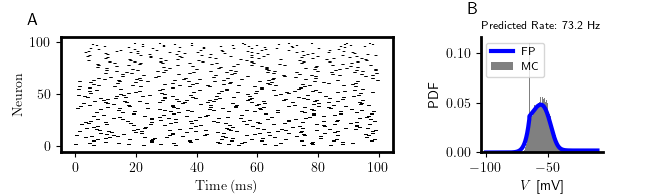
\includegraphics[width=140mm]{figure-3-1}
\end{figure}

Langevin equations have a corresponding Fokker-Planck equation 

\begin{equation*}
\frac{\partial P}{\partial t} = \frac{\sigma^{2}}{\tau}\frac{\partial^{2}P}{\partial V^{2}} + \frac{\partial}{\partial V}\left(\frac{V-E+\psi}{\tau}P\right)
\end{equation*}

\end{frame}


\begin{frame}{Synaptic coupling can induce correlations in spiking activity}

For special synaptic connectivity regimes dynamical variables can remain uncorrelated between neurons

\begin{figure}
\centering
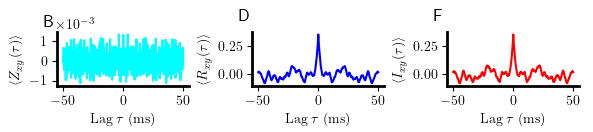
\includegraphics[width=140mm]{figure-12-1}
\end{figure}

Uncorrelated neural activity captures irregular spiking seen \emph{in-vivo}

\end{frame}

\section{Synaptic connectivity as an internal model}
\begin{frame}{Predicting neuron correlations}
The linear response of $r(t)$ allows us to also estimate the matrix of cross-correlations $C_{kj}(\tau)$
from the synaptic connectivity $\mathcal{C}$
\begin{figure}
\centering
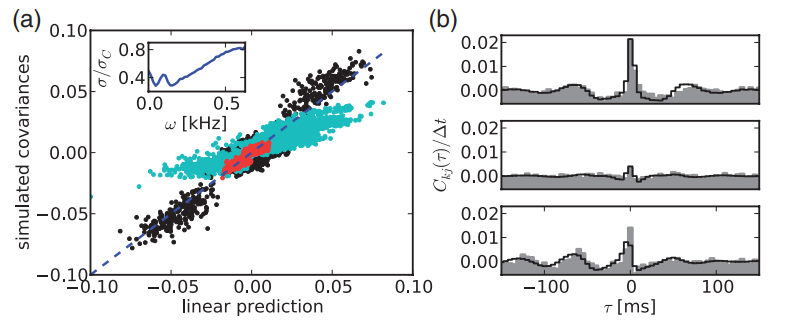
\includegraphics[width=110mm]{figure-20}
\end{figure}

This has important implications for brain-inspired machine learning

\end{frame}


\end{document}